\chapter{A Renewed Case for FPGA-Accelerated Simulation}

To avoid confusion when speaking of computers simulating computers, the
literature commonly makes a distinction between the \emph{target}, the computer
being simulated, and the \emph{host}, the computer executing -- \emph{hosting})
-- the simulation. It is important to note, the host (or more illustrative,
\emph{host-platform}) is often not a single machine, but instead some
collection of interconnected machines, which may include CPUs, GPUs, and FPGAs.

At the time of writing, there is no artifact that completely articulates what
MIDAS is, and what problems it attempts to solve (though, many of core
arguments and ideas are carried over from the RAMP project). Thus, in this
chapter, I attempt to motivate why something like MIDAS is necessary, both for
industrial and academic uses\footnote{It is the view of BAR that this
distinction is to some extent artificial. Good research should lead to
technology transfer.}, before finally describing MIDAS as it exists presently.

\section{A Brief Tour of Full-System Simulation}

Simulation preforms three different functions.

\begin{enumerate}

    \item \textbf{\TODO{Better term - Prototyping}:} ``What thing should we build?" Prototyping
        serves as a means to rapidly evaluate different design points with
        abstract models, or an incomplete implementation of a proposed design.

    \item \textbf{Verification:} ``Did we build the thing right?" Verification
        serves to check (or perhaps, prove) that a particular implementation
        has correctly executes.

    \item \textbf{Validation:} ``Did we build the right thing?" Validation
        serves to show that the implementation fulfills the objectives set out
        for the system.

\end{enumerate}

Both prototyping and verification occurs at all levels of the design hierarchy.
For some specification of the system in which it operates, one could prototype
different accelerators, verify an implementation of the selected design point
in isolation. Validation, however, seeks to answer a system-level question,
that spans the entire computing stack.  The surest way to validate a system, is
not in simulation, but with a physical prototype or the product itself -- but
this pushes validation late into the design cycle. To preform,
\emph{pre-silicon} validation a fast and accurate full-system simulator is
required.

All simulation, full-system or otherwise, makes a tradeoff of between at least
three competing objectives.  \emph{fidelity}~(how accurate is the simulation),
\emph{speed}~(how quickly does simulator execute) and \emph{cost}~(\$ per
simulation hour). \TODO{Table X lists some common technologies are illustrated
in Table X}

Generally, there are only two points during the development of an ASIC in which
full-system simulation, executes within two orders of magnitude of a silicon
implementation. Early in the prototyping phase, where architecture-level
simulators are extended with abstract software models are deployed. And very
late -- when full-system emulation tools a palladium can be used.

For those that cannot afford hardware emulation platform, and those
that want faster simulation sooner, it is common to use an \emph{FPGA
prototype} of the design. FPGA prototypes directly \emph{emulate} the ASIC on
one more more FPGAs, typically with a custom board design that often includes
peripherals identical to what would be deployed in a final product. FPGA
prototypes are fast enough to support software development and thus, a greater
degree pre-silicon validation. Moreover, for a large company, they are
inexpensive enough to build multiple copies that can be more easily shared
between many hardware and software engineering teams.

\subsection{The Full-System Simulation Gap}

The primary difficulty with using both hardware emulators and FPGA prototypes
as full-system simulators, is that they both require complete RTL
implementation of the design. While FPGA-prototypes can accelerate software
development by months, they become useful too late in the design cycle to do
software-hardware co-design, as the hardware platform has been implemented,
limiting the scope of potential changes.

What is truly desired, is a simulator capable of fast and accurate full-system
simulation that can be initially used for early system-prototyping and design
space exploration, into which more detailed models of the machine, and
implementations of it's components can be integrated as they become available.
Here, at all points in the design cycle it is possible to run what exists of
the software on what exists of the hardware design.Thus both hardware and
software design can proceed in parallel, and influence the system specification
early in its design, reducing time to market while producing more aggressive
designs.

\subsection{The Full-System Simulation Gap -- An Academic Perspective}

Academic research in computer architecture is conducted nearly exclusively in
what could be considered the early prototyping phase of the ASIC design cycle.
Full-system software simulation frameworks such as Gem5\cite{gem5}, and
MARSSx86\cite{marssx86} are frequently used by computer architecture
researchers. These simulators can run target workloads at up to hundreds of
KIPS, but are often much slower in practice when employing detailed or custom
models. This makes it practically impossible to run complete workloads, such as
multi-threaded Java applications or SPECint2006~\cite{spec} with its reference
inputs. A common remedy is to employ statistical sampling
techniques~\cite{smarts} to fast-forward to the region of interest, before
executing O(100M) instructions at the desired fidelity.

While this approach has well-acknowledged shortcomings \cite{gem5error},
judicious use of cycle-level simulators can be an appropriate vehicle for
proposing new microarchitectural ideas. But for radical proposals that involve
aggressive microarchitectural changes or traverse multiple layers of the
computing stack, this approach is inadequate (particularly for workloads that
are long-running, irregular and require a large number of cores, such as
managed-language workloads \cite{MicroSimPanel}).

\subsection{Defining FPGA-Accelerated Simulation}

The distinction between FPGA-accelatered simulation and FPGA-prototyping can be
nebulous, especially to those with prior experience in the latter. Here I
argue, that and FPGA-prototype represents a very narrow subset the larger space
of FPGA-accelerated simulation.  The key principal is to, first, abandon the
notion that simulation is special -- a simulation of a computer should
be thought of as an application executing on a host --  and second, forget that a
host may be or include an FPGA.

A simulation is an application that takes an input and produces an output.  The
output may be the console or file I/O of the target machine and a target
wall-clock time. In other cases, it may be a log of all memory requests or
instructions retired. Alternatively, it may be a dump of the state of a module
as it changes over the lifetime of the simulation.  As far as the user is
concerned, the simulation may be optimized in any way whatsover so long as this
output is the same.

Like any other application, simulations have compute intensive kernels that
account for the bulk of the runtime. To improve runtime, the simulation may be
parallelized over that host, either over multiple homogenous resources, or by
offloading specific kernels to \emph{accelerators}, which may execute
concurrently or with the rest of the application.

In simulations that account for time at the cycle-level, much of the runtime is
dedicated to modeling the cycle-by-cycle interactions of parts of the system.
These models may be written in C++ or SystemC, or implemented in an HDL like
verilog or VHDL. Parts of the simulation may be divided into functional models,
like an architecture simulator, and a timing model that does some accounting of
time based on a model of the microarchitecture. What's important to note, is
that any cycle-level model of hardware attempts to capture the behavior of a
fine-grained highly concurrent digital-circuit. Taken to the limit, a
cycle-accurate model completely captures RTL behavior of that circuit.

Unsuprisingly, FPGAs are very good at accelerating kernels with these
characteristics. Thus, in FPGA-accelerated simulation, we attempt to offload
parts of the simulation with these characteristics to an FPGA. One way to
achieve this is to dissolve the simulation spatially (perhaps along module
boundaries): parts of the target, like an NoC or Core pipeline, could be
offloaded to an FPGA, while models for I/O may be hosted on a CPU.
Alternatively, one could host a functional model of a module on the CPU and
accelerate the timing model on the FPGA (or vice versa).  Again, the only
constraint on the implementation of the simulation, and thus, the
implementation of these accelerators, is that as the output of the simulation
is the same. Once this constraint is met, a faster implementation is always better.

Thinking of an FPGA as an accelerator for simulation permits more flexibility
in how FPGAs can be deployed that of FPGA-prototyping. Instead of leaping from
software simulation to prototype, first the software models of the machine are
concretized. Once simulation speed becomes unacceptably slow, FPGA-accelerated
models of key components of the system can be used -- by using a libraries of
FPGA-hosted models that mimic their software counterparts, and with available
RTL. As more of the design is implemented, FPGA-accelerated models of the
implementation can be generated and linked into the simulation. Once the entire
design is implemented, it can be hosted entirely on FPGAs, completing the
transition to FPGA-prototype.

\subsection{Techniques for Building FPGA-Accelerated Simulators}

There is a large body of prior work in academia that have used FPGA as
accelerators~\cite{fast, fame, hasim, protoflex, ramp, diablo}, that have demonstrated
uses of FPGAs that go beyond that of FPGA-prototypes.



%FAME~\cite{fame} presents a taxonomy of FPGA simulators, while cite
%\emph{"FPGA-accelerated Simulation of Computer Systems"}~\cite{fpgasimbook} is
%a more recent, and complete survey of the practise that uses FAST~\cite{FAST}
%and PROTOFlex~\cite{protoflex} as examples. Here 

\subsection{Adoption Challenges}

Despite their promises, FPGA-accelerated simulation has only been successfully employed by
those who designed them. The failure to adopt FPGA-accelerated simulation
methodologies more widely comes as a result of several key factors:

\begin{enumerate}

    \item \textbf{Availability.} Much of the early FPGA simulator research
        relied on boutique FPGA-emulation platforms like the BEE\cite{bee2}, or
        used custom board designs. The cost of these platforms disincentivizes
        their adoption by researchers who already have the means to run
        software simulations at low cost.

    \item \textbf{FPGA Capacity.} Common ASIC structures, such as CAMs and
        multi-ported RAMs, are known to map poorly to FPGA
        fabrics\cite{fpgagap, fpgagap2}, making it difficult to host large
        ASIC designs on an FPGA.

    \item \textbf{Configurability \& Extensibility.} Extending FPGA simulator
        requires writing RTL.
        Previous work\cite{fabscalarfpga, strober} has demonstrated that
        host-decoupled model of the implementation RTL can be transformed from
        source, preserving its RTL behavior while permitting it to be hosted
        in a host-decoupled environment. While this still requires an RTL
        implementation, the same RTL can be used to perform a proper VLSI QoR
        evaluation.

    \item \textbf{FPGA compile time.} Compiling an FPGA simulator takes many
        orders of magnitude longer than compiling a software simulator.
        To some extent this is inescapable. However, where abstract models are
        employed, they can be made run-time configurable, with programmable
        registers sitting on a simulation memory map. Where models are
        generated from RTL, they can can be incrementally recompiled, or perhaps
        partially reconfigured.

    \item \textbf{Debuggability.} Debugging a broken FPGA simulation is
        difficult due to the limited visibility the designer has over the state
        of the simulation. This is strictly more challenging than debugging a
        direct-emulation of the target, as FPGA-specific optimizations make it more
        challenging to reason about the state of the machine.

\end{enumerate}

\subsection{Why Revisit FPGA-Accelerated Simulation?}

Even as Moore's law wanes, FPGA capacity continues to scale. The largest FPGAs
have over 50 MB of BRAM and millions of logic cells\footnote{Comically, scaling
RAMPGold\cite{rampgold}, to use the largest Xilinx UltraScale
FPGA\cite{ultrascale} by BRAM capacity would permit modeling in excess of 5000
cores.}. As they have scaled, FPGAs have continued to become more
heterogeneous, adding features that make them more amenable to hosting
full-system simulators.  Both Intel and Xilinx now sell FPGAs with embedded ARM
cores, making it easier to co-simulate tightly coupled hardware and software
models of a system. Modern FPGAs include hardened DRAM controllers, supporting
memory bandwidth rivaling ASICs. Finally, upcoming Intel Stratix 10 MX parts
include in-package DRAM (HBM2) that can support up to 1 TBps of aggregate
memory bandwidth\cite{stratix10mx}. Both DRAM capacity and bandwidth are
crucial for simulating stateful components of an FPGA-simulator that do not fit
in on-die block RAM.

Lower cost and increased on-chip integration have also made FPGAs more
accessible to researchers.  Not only are commercial off-the-shelf development
boards cheaper and more featured, FPGAs are now available as a service, both
through academic clusters, like TACC's Microsoft
Catapult\cite{catapultannounce} deployment, and through Amazon Web Services'
EC2 F1 instances\cite{amazonf1}. Where in the past academics would have to
purchase their own FPGAs -- even to reproduce published experiments -- it may
soon be possible for them to instead spin up an identical simulation on a
shared computing resource.

\subsection{Improving Usability Through Automation}

While the trends described in the previous section solve the
\emph{availability} and \emph{FPGA capacity} challenges, usability remains a
problem. Previous work\cite{fabscalarfpga, strober} has shown that must of an
FPGA-Accelerated simulator can be automatically generated from source RTL. This
RTL can be written in an HDL like Verilog, or generated from higher-level
frameworks such as Chisel, Bluespec or high-level synthesis tools.

However, there are cases when it is difficult or impossible to automatically
generate models from source RTL. One example are off-chip memory systems: they
cannot be hosted in fabric and yet they must must be tightly coupled to the
processor model.\footnote{High-latency peripherals, like disks, can often be
modeled in software without any performance cost.\cite{disksim}} These
components typically require an abstract model that virtualizes the target
memory system over some extant hardware connected to the FPGA-host. This
reintroduces the aforementioned problem that anything but a simplistic model is
difficult to design, modify and reuse.

We propose to address this through \emph{generators} that synthesize abstract
memory system models that can be easily modified and used across a wide range
of target machines. Such a model must provide a variety of timing models so as
to enable the designer to trade fidelity for FPGA area when needed. It must
also be reconfigurable, to permit sweeping memory system parameters without
needing to recompile the FPGA bitstream. Finally, it must provide useful
instrumentation to both aid in debugging and to provide insight about memory
system behavior without perturbing execution.

\clearpage
\section{An Overview of MIDAS}

We prototype our models in an FPGA-Accelerated simulation framework that builds on
the Rocket-Chip \cite{rocketchip} infrastructure (similar to
\cite{strober}). Our designs are developed in Chisel, a high-level
hardware-description language written in Scala. Building on this infrastructure
allows us to leverage a large amount of available open-source IP and a growing
software ecosystem that includes GCC, Linux and LLVM.

Our framework makes use of FIRRTL~\cite{firrtl}, an intermediate representation
(IR) for RTL that has frontends for both Chisel and Verilog, and can target
both FPGA and ASIC flows by emitting optimized Verilog output. FIRRTL enables
the implementation of compiler passes on top its IR framework. These passes
can, for example, apply FPGA-optimizations, add instrumentation, and
automatically produce scan chains for debugging and power
estimation\cite{strober} -- all without requiring modifications to the source
RTL.

\begin{figure}
	\centering
	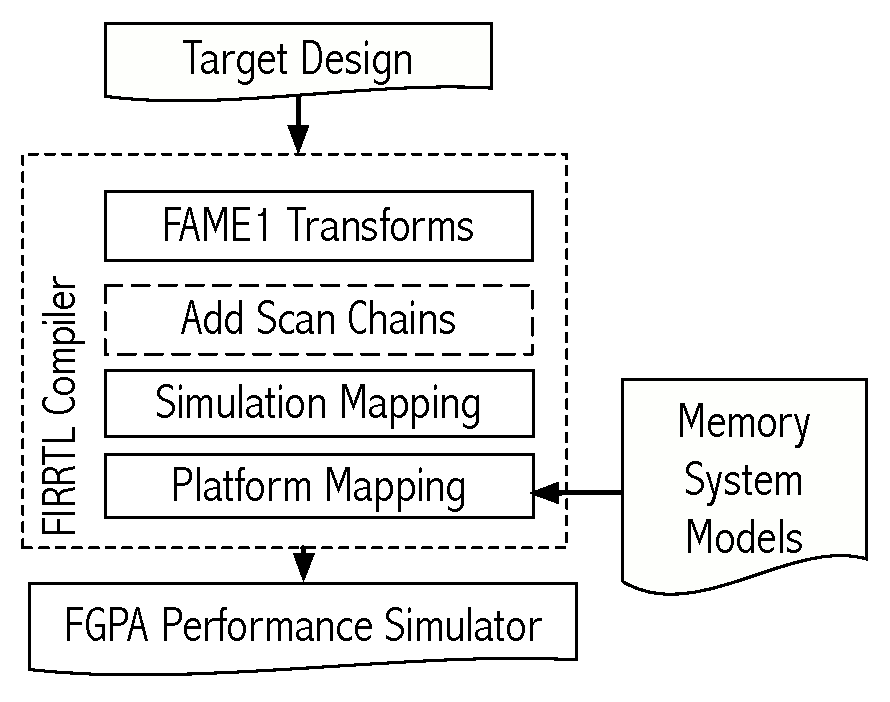
\includegraphics[width=7cm]{figures/firrtl.pdf}
	\caption{FIRRTL custom transforms for the FPGA simulator}
	\label{fig:firrtl}
\end{figure}


\subsection{Host-Target Decoupling in MIDAS}

\subsection{Transformations of Source RTL}

MIDAS uses FIRRTL compiler passes to preform transformation source RTL into
host-decoupled models. The most important of these is the FAME-1
transformation, which adds to requsite logic to host-decouple target RTL, so
that it may conform to a RAMP model of execution. \TODO{See Section}. In figure
\TODO{Auto-transformation} below, the procedure through which source RTL is
host decoupled is illustated.


Additional transformations may be invoked to add scan
chains and I/O trace buffers for debugging, and for state snapshotting for use
with Strober\cite{strober}.

\subsection{Platform Mapping}

\subsection{Target Machines}

While this approach is applicable to arbitrary RTL, one challenge lies in
sourcing the RTL to build a realistic target. While we build on RocketChip and
\RISCV, our approach could in principle be used with other open-source designs
such as OpenPiton\cite{openpiton} and FabScalar\cite{fabscalar}.


\clearpage
\section{An Overview of Off-Chip Memory Systems \& DRAM}

We will now review important first-order architectural
characteristics of DRAM memory-systems that we model in our initial set of
timing models.

\subsection{DRAM Device Architecture}
In a DRAM IC, arrays of bit cells are hierarchically arranged into multiple
parallel \emph{banks}. Banks provide the primitive level of concurrency in a
DRAM memory system. They can service independent requests, assuming they do not
simultaneously require shared resources like the data, address and command
buses.  Multiple DRAM ICs can be arranged in parallel to widen the data bus;
address and command buses fan out to each IC.

A basic DRAM operation requires a series of three commands: \emph{activate
(ACT)}, \emph{column access (CAS)}, and \emph{precharge (PRE)}. The ACT
command enables the word-lines of the array corresponding to a single
\emph{row} of the bank. The cells of the row are sensed and saved in a
\emph{row buffer}(typically O(1) kB). A CAS command then selects a subset of
the row buffer to read or write; data is bursted over successive clock edges.
While the row buffer remains \emph{open}, the row can be accessed by issuing
new CAS commands. To access a row not stored in the buffer, a PRE command must
be issued to \emph{close} the row and charge the bit-lines for a new access.

\subsection{DRAM Controller Architecture}

At the highest level, a DRAM controller is responsible for responding to memory
requests from one or more requestors by scheduling those requests over its
attached memories as a judicious stream of DRAM commands.

Memory access scheduling (MAS) is the process by which, for a given cycle, a
controller selects a single DRAM command to be issued from a legal set. Legal
commands are constrained by the current state of each bank, the availability
of shared resources like the command and data buses, and timing constraints
imposed by the DRAM standard. Good MAS policies strike a delicate balance
between minimizing latency, maintaining quality-of-service guarantees across
multiple threads of execution, maximizing bandwidth, and minimizing power.
There are plethora of academic papers on MAS policies, and still more
industrial patents on the subject. We outline some of the most popular MAS policies
here.

\subsubsection{First-Come First-Serve (FCFS) Policy}\label{fcfs}
Commands for the oldest pending memory reference are always issued first. This
is the simplest MAS policy, but one that grossly under-utilizes available DRAM
bandwidth. FCFS schedulers are common in older machines, and those that present
few concurrent memory requests.

\subsubsection{First-Ready FCFS (FR-FCFS)\cite{frfcfs} Policy}\label{frfcfs}
First, column access commands that hit in an open row-buffer are prioritized,
then row and precharge commands from the oldest pending reference are
considered.  FR-FCFS is a relatively simple scheme that achieves far higher BW
than FCFS. It is the defacto standard against which new MAS policies for
machines with a single stream of memory references (like single-core
out-of-order machines), are compared.

\subsection{System Integration of Off-Chip Memory Systems}


\subsection{DRAM Software Simulation}

The current state of the art in DRAM simulation in academia are cycle-accurate
software simulators like DRAMSim2\cite{dramsim}, Ramulator\cite{ramulator} and
USIMM\cite{usimm}. These models generate DRAM command streams that have been
validated against industrial models (for some standards). Both Ramulator and
DRAMSim2 can be easily integrated into Gem5\cite{gem5}, though it includes a
detailed event-based model of its own\cite{gem5event}. In trace-driven mode,
operating at full throughput and only as a timing model, these cycle-accurate
models simulate at frequencies ranging from 100s of KHz to ones of
MHz\cite{ramulator}.

\subsection{DRAM Power Modeling}

In order to model power, Ramulator relies on DRAMPower\cite{drampower}, to
which it passes its command trace. Micron describes strategies in their
technical notes for estimating DRAM power\cite{micronpower} (which DRAMSim2
employs). They also made these calculations accessible by providing
spreadsheets that take micro-architectural event frequencies as input. These
approaches can carry over to FPGA simulation, as sufficiently detailed FPGA
models can add instrumentation for these events, while simpler models can save
the memory access trace to a buffer and compute power
out-of-band\cite{strober}.
